\documentclass{sig-alternate-05-2015}
\graphicspath{ {./images/} }

\makeatletter
\def\@copyrightspace{\relax}
\makeatother

\begin{document}

\setcopyright{acmcopyright}

\title{Multi-Agent AI}
\subtitle{[Group Coursework 1]}

\numberofauthors{3}
\author{
\alignauthor
Aksel Cakmak\\
       \affaddr{15047472}\\
       \email{zcababc@ucl.ac.uk}
% 2nd. author
\alignauthor
Chong Yang\\
       \affaddr{18089022}\\
       \email{ucabcya@ucl.ac.uk}
% 3rd. author
\alignauthor
Chen Song \\
       \affaddr{17040773}\\
       \email{ucabcs3@ucl.ac.uk}
}

\maketitle

\section{Introduction}

Here we introduce the problem, and present the setting.

Real-time bidding (RTB) offers advertisers a way to adaptively bid for ads on a per-impression basis, in real time.
It uses data from the user's context (cookies, meta-data like the browser used, the website visited, etc..) to formulate a bid price for a certain slot.

If the auction is won, the bidder's ad is then displayed in the slot. Afterwards, the user might or might not click on the displayed ad.

RTB differs from Sponsored Search Auctions, wherein an auction mechanism tries to match advertisers that bid on certain search keywords, not on specific impressions.

Bidders have a certain budget to allocate to a certain number of bids, and (in our specific setting) want to maximise the total number of clicks they get from all the ads they display.

For a specific slot, the bidder is usually interested in some specific KPI (key performance indicator) that they use to formulate their bid (in our case, we're interested in the predicted click-through-rate of a specific slot, or pCTR).

Then, a bidder has the following dimensions to consider for its bidding campaign: \\
- How to predict the KPI (here, pCTR), the choice of a predictive model, its accuracy, etc.. \\
- How the bid is formulated wrt a given pCTR. \\

The bidder wants to optimise the number of clicks it gets by choosing a good KPI predicting model and a good bidding function (in our specific setting).
In addition to this, one other constraint there is is that the whole pipeline of KPI prediction + bid function has to be calculated with minimal latency (bids often have to be submitted within a short timeframe, like 100ms) \cite{MILLI, PHD1}.


\section{Approach and Results}

%%%%%
\subsection{Problem 1: Data Exploration and Literature Review}

\subsubsection{Literature Review}


The performance of a CTR prediction model has a direct impact on the final number of clicks generated by a campaign,
which is why a lot of work has been made on how to predict the CTR of a given slot.

Regularised Logistic Regression model have been commonly used for the task of predicting CTR \cite{LOGREG1}, but are lacking in that they require some feature engineering work and are not as accurate as newer Deep Learning based methods. \cite{DL1}

As a consequence, more Deep Learning based methods have been proposed recently, where the input features are fed into neural networks which learn the implicit nonlinear relations between the different features, and consequently report enhanced accuracies. \cite{DL2, DL3, DL5} 

Once the pipeline has a model to predict the CTR, there exist different approaches to calculating a bid wrt this pCTR.



Some very simple approaches include bidding a constant value, or choosing a random bid based on some range.
Quite naturally, these approaches don't fare as well as other more sophisticated methods, that bid a variable amount using the pCTR and the contextual information of a specific slot.  \cite{ORTB}
One more advanced approach is linear bidding: the bidding value is an affine function of the predicted CTR (pCTR).
This method fares far better than the aforementioned, but is outclassed by non-linear methods like \cite{ORTB}.

% more details on the specific models ? or leave that to the actual relevant sections ?

One challenge of this particular setting is that the bidding is budget constrained: 
the advertiser (in our setting) wants to maximize the number of clicks it gets from its impressions, for some number of slots it bids for.
Knowing how fast one should burn through the given budget is a difficult problem\cite{BID1}:
If the strategy bids relatively high values, the budget might be spent early and some potentially valuable slots might be missed.
If the strategy is relatively more conservative, then the budget might not be fully spent and some valuable slots might be underbid on.
The problem is even more complex when considering the fact that there are a number of heterogeneous and unpredictable other agents with their own bidding strategies competing against a given bidder. \cite{BID1}
Determining the best rate of spending is an open question. \cite{OPENQ}



\subsubsection{Data Exploration}

look at the paper he advised
get something working with the stats he did
at least a couple of them
with some commentary


%%%%
\subsection{Problem 2: Basic Bidding Strategy}
In this section, we analyse two basic bidding strategies, which are Constant Bidding Strategy and Random Bidding Strategy, and evaluate their performance based on the number of clicks within a limited budget of 6,250 CNY fen. 
Evaluation function: For the single-agent basic bidding strategies, the main metric to rank the strategies are based on the clicks from winning impressions.

\subsubsection{Constant Bidding Strategy}
In order to find an optimal constant value, we loop the constant bid prices from 0 to 300, which are the minimum bid price and maximum bid price, to find out the bid price with the highest clicks from winning impressions. Specifically, for each constant price, we retrieve the columns of 'payprice' and 'click' for all the bids in the training set. Then we compare our constant bid price with the 'payprice' for each bid and add up the click into our total clicks if our constant bid price is great than or equal to the 'payprice' while the total spend is calculated at the mean time. Afterwards we remove the clicks from bottom to top where the total spend has been over our limited budget.

Analysis: 
Figure 1 shows that how the number of clicks changes based on the increment of the constant bidding price.
The clicks increase dramatically when the constant bidding price increases from 1 to 24 and the climax of clicks is 134 when the constant bidding price is 24. Then the clicks drop sharply when the bidding price increases from 25 to 69. Afterwards, the clicks decrease smoothly.

In order to evaluate our result on validation set, initially we need to normalise the budget based on the Equation 1.\\

\begin{equation}bidPrice_{validation}=\frac{sizeOfValidation}{sizeOfTrain} * bidPrice_{train}\end{equation}


Figure 2 shows the changes of number of clicks depending on bid price in the validation set with a normalised budget. We could see the clicks are relatively high when the bid price is between 18 to 68. Moreover, the highest clicks are 15 while the clicks are 12 when bid price is 24. Therefore, bid price 24 is a relatively satisfactory price in the validation set.

\begin{figure}
\centering
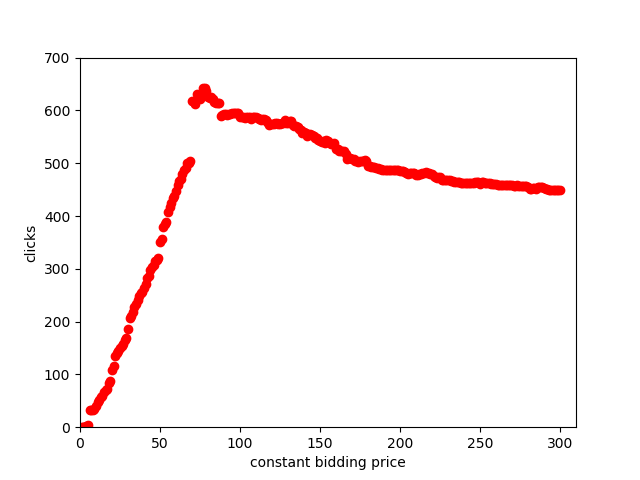
\includegraphics[height=2in, width=2in]{images/constant_bidding.png}
\caption{Validation set - bid price and clicks}
\end{figure}

\begin{figure}
\centering
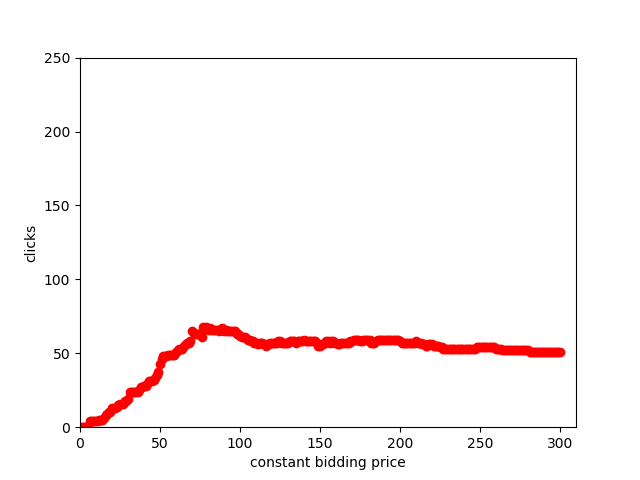
\includegraphics[height=2in, width=2in]{images/constant_bidding_validation.png}
\caption{Validation set - bid price and clicks}
\end{figure}




\subsubsection{Random Bidding Strategy}
In order to find the optimal bidding range for random bidding, we step through a range of lower bound and a range of upper bound to find out the bid price with the highest clicks from winning impressions. Similarly, we use the same method as the one in Constant Bidding Strategy to calculate the clicks. 

Analysis: 
The highest clicks are 132 generated from range(30, 40) and the second highest clicks are 131 generated by range(0, 50) in the training set. By normalising the budget in the validation set based on equation 1, we find the highest clicks are 15 generated from the range(0, 50). Therefore, the findings in training set successfully match validation set. 

\subsubsection{Competition among homogeneous random bidding agents}

%%%%%
\subsection{Problem 3: Linear Bidding Strategy}
In order to apply CTR estimation to for a linear bidding strategy, we initially retrieve the these features as independent variables X: day, hour, region, ad exchange, slot width, slot height, advertiser, slot visibility, slot format, OS, browser, and slot price from the data set. Specifically, we categorise the slot price to five categories based on the price values, and we extract the OS and browser from the column useragent. And the rest features could be simply fetched from the data. The click from the data is our predictor Y.
Afterwards, we import the Logistic Regression model from sklearn and train the model with the independent variables and predictor from the training set. Then we use the trained model to predict the click of test data and validation data separately. The pCTR of the validation data could be calculated with the equation 2.
\begin{equation}pCTR=\frac{numOfClicks}{numOfWinningImpressions}\end{equation}

The bid price for each bid is calculated as equation 3. As shown in Figure 3, the total clicks increase sharply when base bid increases from 1 to 20 and drop smoothly after then. The value clicks is maximised as 39 when the base bid is 20.

\begin{equation}bidPrice=\frac{baseBidPrice*pCTR}{avgCTR}\end{equation}

\begin{figure}
\centering
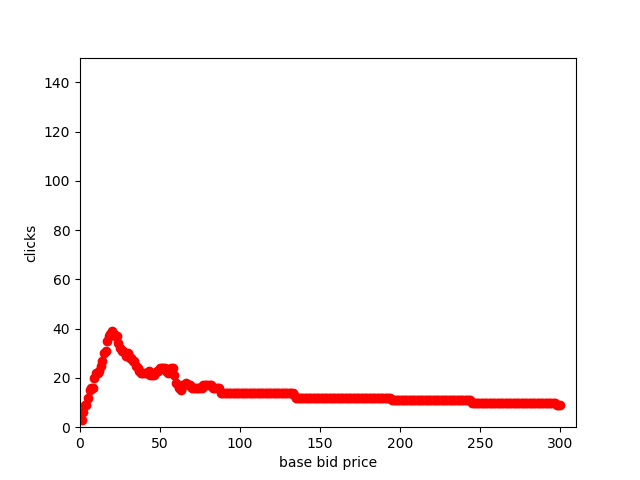
\includegraphics[height=2in, width=2in]{images/base_bid_price.png}
\caption{Validation set - base price and clicks}
\end{figure}

Comparison:
\begin{table}
\centering
\caption{Behaviour Comparison}
\begin{tabular}{|c|c|c|l|} \hline
&Constant Bidding&Random Bidding&Linear Bidding\\ \hline
price&24&range(0, 50)&20(base)\\ \hline
clicks&12& 15&39\\
\hline\end{tabular}
\end{table}

Obviously, the behaviour of the linear bidding strategy is much better than random bidding and constant bidding strategies. The optimal value of clicks in linear bidding is 39 while the ones of constant bidding and random bidding are merely 12 and 15 separately.

%%%%%%%
\subsection{Problem 4: Non-Linear Bidding Strategy}
We calculate the non-linear bidding price based on ORTB (equation 4), and we step through some combination of c and lambda to find the optimal pair generating the optimal bid prices. We find the value of clicks is 39 when c equals to 39 and lambda equals to 1.31072e-05. Therefore, our non-linear bidding strategy just generates the same result as linear bidding strategy.
\begin{equation}bidPrice=\sqrt{\frac{c}{\lambda} * pCTR + c^2} - c\end{equation}


%%%%%%%
\subsection{Problem 5: Multi-agent Bidding Strategy}

\section{Conclusions}
This paragraph will end the body of this sample document.
Remember that you might still have Acknowledgments or
Appendices; brief samples of these
follow.








%
%\subsection{Citations}
%Citations to articles \cite{bowman:reasoning,
%clark:pct, braams:babel, herlihy:methodology},
%conference proceedings \cite{clark:pct} or
%books \cite{salas:calculus, Lamport:LaTeX}




\bibliographystyle{abbrv}
\bibliography{sigproc}
\begin{thebibliography}{9}

\bibitem{LOGREG1} 
H. Brendan Mcmahan, H. Brendan Holt, et al. 2014. 
Ad Click Prediction: a View from the Trenches. 
In Proceedings of the 19th ACM SIGKDD International Conference on Knowledge Discovery and Data Mining. 1222?1230.

\bibitem{PHD1} 
Weinan Zhang et al. 2014.
Optimal real-time bidding for display advertising.
Proceedings of the 20th ACM SIGKDD international conference on Knowledge discovery and data mining.

\bibitem{DL1} 
Guorui Zhou et al. 
Deep Interest Network for Click-Through Rate Prediction.
In Proceedings of the 24th ACM SIGKDD International Conference on Knowledge Discovery \& Data Mining.

\bibitem{DL2}
Paul Covington, Jay Adams, and Emre Sargin. 2016. 
Deep neural networks for youtube recommendations. 
In Proceedings of the 10th ACM Conference on Recommender Systems. ACM, 191?198.

\bibitem{DL3}
Cheng H. et al. 2016. Wide \& deep learning for recommender systems. 
In Proceedings of the 1st Workshop on Deep Learning for Recommender Systems. ACM.

\bibitem{DL4}
Ying Shan, T Ryan Hoens, Jian Jiao, Haijing Wang, Dong Yu, and JC Mao. Deep
Crossing: Web-scale modeling without manually crafted combinatorial features.

\bibitem{DL5}
Shuangfei Zhai, Keng-hao Chang, Ruofei Zhang, and Zhongfei Mark Zhang. 2016.
Deepintent: Learning attentions for online advertising with recurrent neural networks. 
In Proceedings of the 22nd ACM SIGKDD International Conference on Knowledge Discovery and Data Mining. ACM, 1295?1304.

\bibitem{MILLI}
Shuai Yuan, Jun Wang, and Xiaoxue Zhao. Real-time bidding for online advertising: measurement and analysis. 
In Proceedings of the Seventh International Workshop on Data Mining for Online Advertising, page 3. ACM, 2013.

\bibitem{ORTB}
Weinan Zhang, Shuai Yuan, and Jun Wang. Optimal real-time bidding for display advertising. 
In Proceedings of the 20th ACM SIGKDD international conference on Knowledge discovery and data mining, pages 1077?1086. ACM, 2014.

\end{thebibliography}


\end{document}






